
\chapter{Fundamentação Teórica}
\label{fundamentacao-teorica}

\section{Geomarketing}
\label{Geom}
Segundo \citeonline{Sergio2005}, \emph{geomarketing} é o nome dado à área de
gerenciamento de informação que incorpora as dimensões espaciais para auxiliar a
tomada de decisões dentro de um domínio específico de mercado, o que permite
levantar as características de uma determinada região e analisar seu potencial
sócio-econômico. Pode ser entendido, assim, como uma ferramenta de análise
estatística de dados, com intuito de localizar padrões que possam ser utilizados
e combinados na elaboração de indicadores, perfis de consumo e estratégias de
negócios, de modo a gerar informação relevante na tomada de decisões.
Geralmente, o serviço é oferecido por consultorias especializadas - o  objetivo
da empresa  contratante é a melhoria no desempenho de seu negócio.

\subsection{Casos de uso}
O termo \emph{geomarketing} é ainda pouco conhecido no Brasil, no entanto cada
vez mais se populariza no âmbito dos negócios. Segundo a revista
\citeonline{Exame}, utilizado de forma amadora há 20 anos, o uso de ferramentas
de localização geográfica evoluiu e alcançou importância dentro da estratégia de
expansão das empresas - grupos como Coca-Cola e O Boticário usam o marketing
geográfico. Pequenas e médias empresas já começam a mirar em sistemas de busca
com foco na geolocalização. Podemos citar como exemplo de pequeno negócio que
empregou o \emph{geomarketing} um restaurante voltado à alimentação saudável em
Natal-RN - o objetivo foi verificar a distribuição geográfica de clientes e
mapear áreas de influência para conhecer melhor a demanda do mercado. De acordo
com \citeonline{Seabra2014}, esta investigação permitiu uma compreensão do
fenômeno da área de influência e de variáveis que modelam seu comportamento. O
estudo baseou-se em informações obtidas através de softwares como Google
Maps para o georreferenciamento e análise dos dados - isso só foi possível
graças a fácil disponibilidade e barateamento da tecnologia atual: o
Google Maps é um exemplo de ferramenta de geolocalização bastante popular
e acessível que, há alguns anos, não existia.

Por outro lado, o acelerado desenvolvimento tecnológico e o crescimento de
grandes centros urbanos criaram uma infinidade de possibilidades em aplicações
para o \emph{geomarketing}, tornando a ferramenta cada vez mais ampla e
complexa. Um exemplo a ser citado nesse contexto é a aplicação do
\emph{geomarketing} como ferramenta de análise para criação de novas estações na
CPTM (Companhia Paulista de Trens Metropolitanos). Segundo
\citeonline{Mangini2014}, o modelo apresentou ser de grande valia por reduzir de
forma substancial a subjetividade da escolha do local para uma nova estação e
pôde ainda ser utilizado como método para a definição de novas linhas férreas.

Podemos assim perceber a dimensão e importância do \emph{geomarketing} hoje como
referencial na tomada de decisões estratégias em organizações,
tornando-o aos gestores uma ferramenta valiosa, a qual pode significar a
diferença entre sucesso ou fracasso de um negócio.

\subsection{Tráfego de pessoas e o geomarketing}
Diante do exposto na \autoref{Geom}, o presente trabalho
visa utilizar conceitos de \emph{geomarketing} e dispositivos móveis na
verificação do tráfego de pessoas em áreas específicas, permitindo organizações analisarem a
demanda de acordo com a sua necessidade, também podendo avaliar a entrada
de novos pontos estratégicos de atuação ou mesmo incrementar o alcance nos
locais já existentes. Um exemplo de público-alvo poderia ser representado por
\emph{shopping centers}, restaurantes, franquias, etc.

\section{Ferramentas de contagem de pessoas}
Para que o \emph{geomarketing} e o tráfego de pessoas sejam implementados, é necessário medir o número
de pessoas através de uma ferramenta de contagem.

As ferramentas de contagens de pessoas
são sistemas eletrônicos que utilizam leitores para contar as pessoas
\cite{trafsysdef}. O tráfego de pessoas é gerado por essa contagem durante
certos períodos de tempo. Estas informações quando aliadas com outras métricas de
negócio proporciona a gestores informações estratégicas.

\subsection{Tipos de contadores}
Não existe apenas um método para contar o número de pessoas. As principais
diferenças entre os contadores estão em: área de cobertura, volume e tecnologia
utilizada. Segundo \citeonline{wikipedia2017} e \citeonline{Ipsos} os principais métodos de
contagem são:

\begin{itemize}
  \item \textbf{Feixes infravermelhos:} são colocados
na entrada de lojas emitindo um feixe infravermelho entre os seus extremos,
quando alguém interrompe o feixe, uma entrada é contada. A área de cobertura é
pequena e o volume de pessoas que ele permite passando pela porta ao mesmo
tempo é baixíssima;
  \item \textbf{Câmeras termais:} o uso de sensores térmicos e
processamento de imagens. Normalmente,
são posicionados no teto para que a imagem capture a temperatura das pessoas
e compare com a do ambiente. Este sistema permite alto volume de tráfego e instalação em entradas complexas;
  \item \textbf{Vídeo:} Utilização de algoritmos complexos, inteligência artificial
   e o processamento de imagens (2D e 3D). A área de cobertura
  pode ser medida de acordo com o uso de câmeras e o volume permitido varia de acordo com os algoritmos;
  \item \textbf{Wi-Fi:} utiliza o receptor Wi-Fi para pegar \emph{frames} únicos de gerenciamento Wi-Fi emitidos por dispositivos
  dentro do alcance. Ideal para áreas onde o volume de pessoas é esparso ou incerto.
\end{itemize}

A escolha de um contador varia de acordo com a complexidade da entrada do lugar, períodos de captura do tráfego de pessoas,
volume de pessoas por período, área de cobertura, precisão desejada, preço, entre outros \cite{trafsys} \cite{Axper2017}.

\subsection{Área acadêmica}
A principal técnica de contagem de pessoas pesquisada é por câmeras e processamento de imagens. Entretanto,
as pesquisas diferenciam-se por técnicas de computação utilizadas. Alguns exemplos são:

\begin{itemize}

  \item \textbf{Robusto e leve:} com o objetivo de fornecer segurança para ambientes internos
  o trabalho de \citeonline{Kim2002} preza por um sistema que seja robusto suficiente para garantir as metas, mas
  não seja tão pesado do ponto de vista de algoritmos e demanda de hardware. O sistema reconhece o movimento de pessoas
  ao longo de várias direções através de uma única câmera e um processador Pentium IV, assim ele estima e rastreia uma "caixa"  ao redor de cada indivíduo
  para identificá-lo na imagem;

  \item \textbf{Melhora no processamento de imagens e ruídos:} as pesquisas de \citeonline{Luo2016} e \citeonline{Hou2011} consideram
  a queda de desempenho de sistemas de contagem em ambientes com multidões, oclusões (sombreamento/luminosidade
  em cada quadro do vídeo) e informações de fundo complexas. O primeiro artigo propõe uma abordagem de cenas \emph{indoor}
  que leva em conta multidões estacionárias (paradas) ou em movimento. O sistema detecta a multidão e separa
  os ruídos. Depois, estima-se o número de pessoas através de "ombro-cabeça". Por fim, para reduzir as oclusões,
  há um filtro que separa quadro por quadro do vídeo e faz um tratamento. Já o segundo, foca em subtrair o fundo, estima
  o número de pessoas e utiliza técnicas para identificar as pessoas em imagens de baixa resolução;

  \item \textbf{Múltiplos recursos:} os artigos de \citeonline{Venkatesh2015} e \citeonline{Ma2012} consideram múltiplos recursos para contar pessoas
  em ambientes densos. O primeiro utiliza, principalmente, técnicas matemáticas e técnicas de filtros e imagens para estimar. Já o segundo, utiliza
  múltiplas câmeras e vários níveis de textura para lidar com aparência humana e posições.

\end{itemize}

  As principais caraterísticas de sistemas de contagem que os artigos levantados focaram e presaram foram: movimentação das pessoas,
  ambientes de multidão e processamento em tempo real.

\subsection{Produtos na área empresarial}
\label{produtos-empresas}
Esta seção apresenta alguns contadores de algumas empresas. Na \autoref{density}, a empresa Density oferece a contagem a partir de um
dispositivo localizado no topo da entrada que processa imagens 2D \cite{Density2017}. Já na \autoref{axper}, a empresa Axper além de oferecer
o processamento de imagens 2D como a Density, oferece também um dispositivo que processa imagens 3D, cobrindo todo o ambiente \cite{Axper2017}.

\begin{figure}[htb]
  \caption{\label{density}Processamento de imagens 2D - Density People Counter}
  \begin{center}
    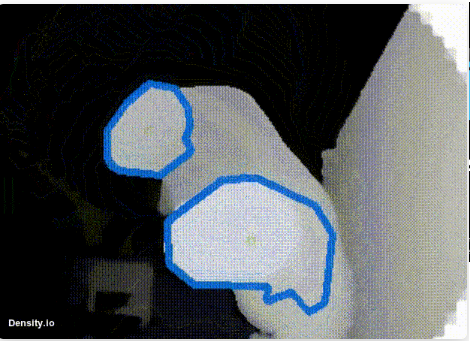
\includegraphics[width=0.40\textwidth]{img/density.png}
  \end{center}
  \legend{Fonte: \citeonline{Density2017}.}
\end{figure}

\begin{figure}[htb]
  \caption{\label{axper}Processamento de imagens 2D e 3D - Axper People Counter}
  \begin{center}
    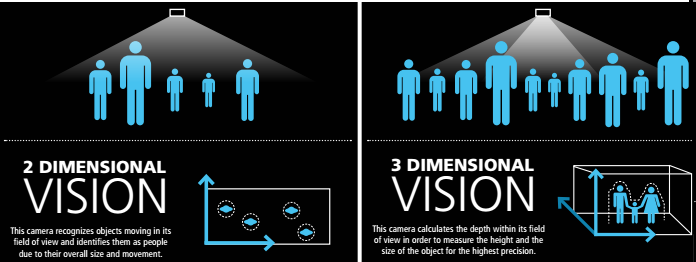
\includegraphics[width=0.70\textwidth]{img/axper.png}
  \end{center}
  \legend{Fonte: \citeonline{Axper2017}.}
\end{figure}

A empresa \citeonline{V-Count2017} oferece soluções de contagem a partir de imagens termais e sinais Wi-Fi. Na \autoref{v-count1}, a contagem ocorre por um
aparelho fixado na entrada da loja que recebe sinais dos dispositivos móveis das pessoas que passam em frente. Já a \autoref{v-count2}
mostra as soluções que processam imagens e a temperatura para identificar os clientes e seus hábitos.

\begin{figure}[htb]
  \caption{\label{v-count1}Street Counting - V-Counter}
  \begin{center}
    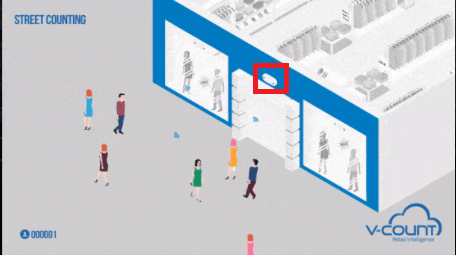
\includegraphics[width=0.70\textwidth]{img/v-count.png}
  \end{center}
  \legend{Fonte: \citeonline{V-Count2017}.}
\end{figure}

\begin{figure}[htb]
  \caption{\label{v-count2}Visitor Counting e Camera Heatmap - V-Counter}
  \begin{center}
    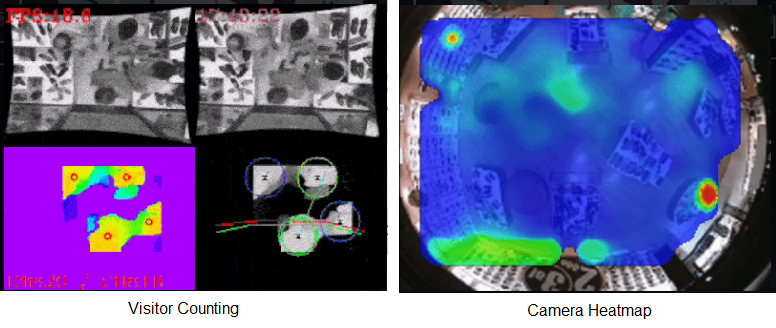
\includegraphics[width=0.70\textwidth]{img/termal-vcount.png}
  \end{center}
  \legend{Fonte: \citeonline{V-Count2017}.}
\end{figure}

%\subsection{Motivos de adoção} ISSo AQUI VAMOS COLOCAR DEPOIS SE NÃO NAO DÀ TEMPO
%Os motivos que levam uma organização a adotar as ferramentas de contagem de pessoas são:
\subsection{Escolha da forma de contagem}
Foi observado que as principais pesquisas de técnicas para a contagem de pessoas abordam o processamento de imagens e vídeo. Já no âmbito empresarial,
há diversificadas soluções partindo desde o uso dessas imagens até o uso de emissão de sinais Wi-Fi.
As soluções em TI que empregam as redes sem fio para identificar pessoas são variadas. Por exemplo,
uma área amplamente explorada em pesquisas é a localização de pessoas em
ambientes fechados (\emph{indoor location}) que utiliza dispositivos móveis e emissão de sinais \emph{wireless} \cite{Ferreira2016}
\cite{Puhl2016} \cite{Figuera2011}. No entanto, o uso da técnica de contagem por Wi-Fi como ferramenta do \emph{geomarketing} não
é amplamente desenvolvida na comunidade aberta, estando restrita principalmente a empresas de consultoria e serviços de TI, como citadas
na \autoref{produtos-empresas}.

Visto a baixa exploração do uso do Wi-Fi como ferramenta de \emph{geomarketing} em comunidade aberta, este trabalho pretende
desenvolver um sistema que empregue esse tipo de comunicação para a contagem e identificação de pessoas e seus perfis. A escolha da comunicação
sem fio ocorreu também devido sua grande área de cobertura, pois o tema de identificar indivíduos
em multidões foi apontado como tendência de pesquisa.


\section{Número e uso de dispositivos}

A abundância de dispositivos móveis por pessoas tende a crescer cada vez mais. Segundo a \citeonline{Ciscoblogs} até 2013, havia 80 dispositivos
se conectando por segundo na Internet, e até 2020 serão 250 se conectando. Ainda nessa pesquisa, revela-se que haverão em média
50 bilhões de dispositivos conectados até 2020. Já a \citeonline{Gartner2014} estima que até 2020 haverão 20.8 milhões de dispositivos.
Até o final de 2016 foram estimados 6,4 bilhões de dispositivos conectados \cite{Gartner2014}. Como pode ser visto, a \autoref{cisco2011}
revela que até 2020 serão quase 7 aparelhos conectados por pessoa.

\begin{figure}[htb]
  \caption{\label{cisco2011}Número de dispositivos conectados - Cisco IBSG 2011}
  \begin{center}
    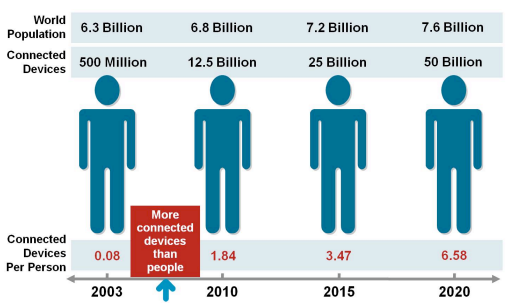
\includegraphics[width=0.70\textwidth]{img/cisco-2011.png}
  \end{center}
  \legend{Fonte: \citeonline{Evans2011}.}
\end{figure}

Apesar de expressiva a diferença entre as estimativas anteriores, ambas revelam o aumento do uso de dispositivos conectados.
A pesquisa da \citeonline{Cisco2017a} pode revelar mais sobre o crescimento do uso e o tipo de aparelhos. Segundo essa pesquisa,
como mostra a \autoref{cisco-2017}, desde
2016 até 2021, o maior de tráfego de exabytes por mês é e será de \emph{smartphones}.

\begin{figure}[htb]
  \caption{\label{cisco-2017}Tráfego mundial de dispositivos móveis por tipo}
  \begin{center}
    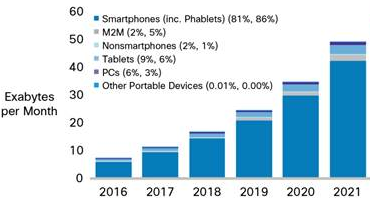
\includegraphics[width=0.70\textwidth]{img/cisco-2017.png}
  \end{center}
  \legend{Fonte: \citeonline{Cisco2017a}.}
\end{figure}

Segundo a \citeonline{Teleco}, na pesquisa da IDC Brasil
no último trimestre de 2016 foram vendidos 48,4 milhões de dispositivos no Brasil, sendo 4,9 milhões de celulares tradicionais e 43,5
milhões de smartphones. Apesar
de haver queda de vendas nos últimos anos de \emph{smartphones}, a proporção de vendas ainda é maior para este tipo de aparelho. Já o total
de celulares no Brasil, em março de 2017, é de aproximadamente 242 milhões, como demonstra a \autoref{dados2017}.

\begin{figure}[htb]
  \caption{\label{dados2017}Quantidade de Celulares no Brasil - Março 2017}
  \begin{center}
    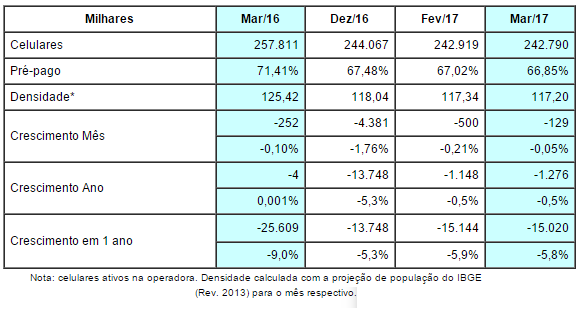
\includegraphics[width=1.0\textwidth]{img/dados2017.png}
  \end{center}
  \legend{Fonte: \citeonline{Teleco}.}
\end{figure}

\section{Dispositivo móvel como objeto identificador}
\label{dispositivo-coisa}
Assim como os RFIDs passivos utilizados em uma cadeia de suprimentos para identificar produtos que vão num caminhão, ou como os códigos de barras
que fornecem ao operador de caixa informações sobre um produto, os dispositivos móveis, como os \emph{smartphones}, serão utilizados
como objetos identificadores neste trabalho. Tendo em vista que a proporção de \emph{smartphones} é maior que a de celulares tradicionais no Brasil e, em
todo o mundo, considera-se esse equipamento de uso comum. Além disso, esses dispositivos móveis fornecem informação pública passiva
através da rede Wi-Fi e independem da fabricante para serem detectados numa rede - portanto, serão utilizados como meio
de identificação das pessoas (\autoref{smartphone-probe}).

\section{Modo Monitor}
\label{modo-monitor}
Para que um dispositivo móvel seja identificado independente de qualquer rede ou AP, é essencial que o sistema de detecção possua uma placa e/ou adaptador de rede (NIC) que possa ser habilitado para o modo monitor.

Geralmente, uma interface de rede qualquer captura pacotes dos tipos \emph{managed} e \emph{beacons} que são originados por APs. Estes pacotes são transmitidos
muitas vezes por segundo por APs para indicar quais redes estão realizando \emph{broadcasting}. O modo monitor (\emph{monitor mode}) é um modo de operação em que um NIC consegue capturar todos os tipos de pacotes sem estar associado a um AP \cite{Acrylic} \cite{Wireshark2017b}. Dessa forma, é possível capturar todos os tipos, como os de \emph{probe request} que são enviados de dispositivos móveis para pontos de acesso para saber quais redes próximas estão disponíveis para se conectar.

Neste trabalho, um Raspberry Pi com um adaptador Wi-Fi habilitado no modo monitor captura pacotes \emph{probe request} de \meph{smartphones}
para que ocorra a identificação de indivíduos (\autoref{smartphone-probe}).

\section{Trabalhos correlatos}
\label{trabalhos-correlatos}
Este subcapítulo apresenta algumas soluções que
empregam a detecção de dispositivos móveis por sinais Wi-Fi e utilizam como ferramenta
de \emph{geomarketing}.

\subsection{Cidade Jardim}

Em 2016, a empresa Zebra Technologies implantou no Shopping Cidade Jardim, em São Paulo, o seu
projeto MPact. Este oferece aos clientes acesso gratuito à Internet e, quando esses indivíduos estão
conectados, consegue a localização do consumidor em três níveis: zona, posição e
presença. Com estas informações, é possível saber sobre uma determinada pessoa:
quem é, onde está, quanto tempo fica em certas áreas e quais produtos está
adquirindo. Utilizando a rede Wi-Fi e Bluetooth, este projeto identifica a
posição e o tempo exato onde cada consumidor se encontra.

O MPact proporciona aos varejistas, lojistas e operadores do shopping melhor
entendimento sobre o comportamento dos consumidores. Por exemplo, é possível
saber quais corredores estão mais cheios, quais lojas estão vendendo mais e
quais pontos mais chamam a atenção, ou seja, este sistema auxilia no
monitoramento de pontos de venda. Segundo a \citeonline{zebra}, esta é uma
maneira de entender o que os clientes querem, para então ganhá-los e mantê-los.

\subsection{Meshlium Xtreme}
O Meshlium Xtreme é um produto da empresa Libelium
que detecta dispositivos móveis e veículos para garantir inteligência de
negócios. Ao detectar dispositivos através de sinais Wi-Fi e Bluetooth, esse
sistema mede pessoas e carros, gerando informações \cite{libelium}. Sobre a
atividade de pessoas as informações são: quantidade de pessoas passando numa rua
diariamente, média de tempo que as pessoas ficam numa rua, diferença entre
visitantes e residentes e rotas de caminhadas pelas lojas. Sobre veículos:
número de veículos em tempo real passando em certo ponto, média de tempo que
veículo fica parado, média de velocidade e tempos de viagem em rotas
alternativas quando congestionamento é detectado.

Os dispositivos detectados não precisam
estar conectados a nenhum AP, possibilitando a detecção de qualquer um
independente da fabricante. Já veículos são detectados até 100 km/h. O objetivo
principal deste produto é medir a quantidade de pessoas e carros num determinado
ponto e uma hora específica, permitindo que sejam tomadas decisões estratégicas
sobre o tráfego de pessoas e carros sobre área específica. As figuras
\autoref{meshlium-celulares} e \autoref{meshlium-carros} demonstram o
funcionamento do produto.

\begin{figure}[htb]
  \caption{\label{meshlium-celulares}Detecção de \emph{smartphones}}
  \begin{center}
    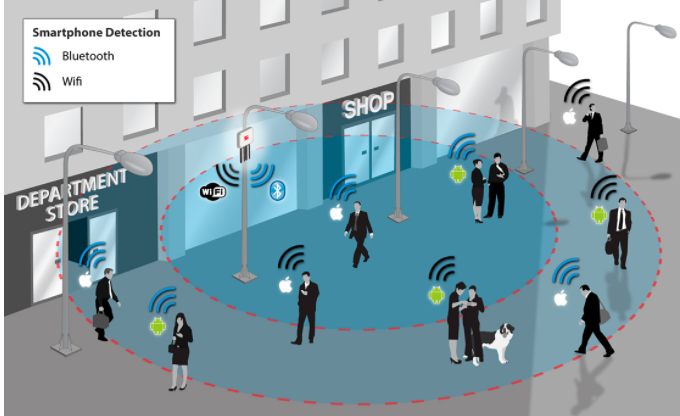
\includegraphics[width=0.60\textwidth]{img/meshlium-celulares.png}
  \end{center}
  \legend{Fonte: \citeonline{libelium}.}
\end{figure}

\begin{figure}[htb]
  \caption{\label{meshlium-carros}Detecção de veículos}
  \begin{center}
    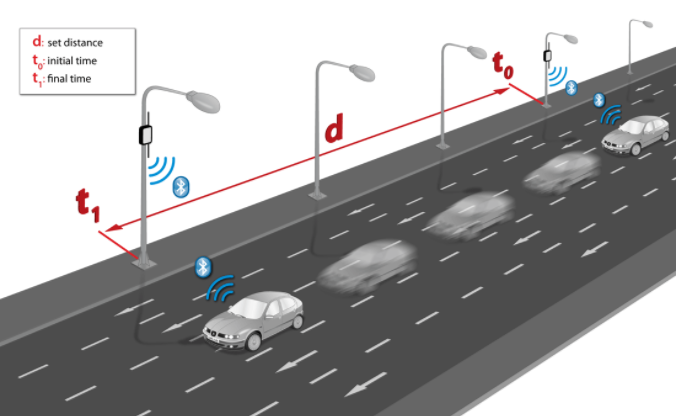
\includegraphics[width=0.60\textwidth]{img/meshlium-carros.png}
  \end{center}
  \legend{Fonte: \citeonline{libelium}.}
\end{figure}

\subsection{How many people are around}
``How many people are around'' (em inglês, quantas pessoas estão ao redor) é um projeto encontrado no Github do usuário \citeonline{Schollz2017} que utiliza um \emph{cluster} de Raspberry Pi's para calcular o número de pessoas próximas e/ou dentro de casa. Para tanto, ele utiliza o protocolo de análise Tshark para detectar Wi-Fi \emph{probe requests} de \emph{smartphones} e a linguagem Python. Além disso, os dados capturados podem ser observados em forma de gráfico.

